% !TEX root = ../thesis.tex

In this chapter, we start with a brief overview of Monte Carlo estimators and associated sampling methods focusing in particular on Sequential Monte Carlo methods for the smoothing and filtering problem on Hidden Markov Models. We also introduce an alternative class of methods relying upon Piecewise Deterministic Markov Processes and in particular the Bouncy Particle Sampler (BPS). 

\section{\label{sec:MC+SMC}Monte Carlo Methods}
In this section we review briefly the foundations of Monte Carlo methods as well as a few key algorithms which will be discussed in the rest of the document.

\subsection{From quadrature to sampling}
% KEEP pi (later p is filtering/smoothing)
We consider the problem of computing the expected value of a test function $\varphi$ taking value over a space $\mathcal X$ with respect to a distribution $\pi\in\mathcal P(\mathcal X)$ i.e.: $I:=\E_\pi[\varphi(X)]$. Assuming it cannot be computed analytically, a general approach is to consider a quadrature rule of the form:
%
\eqa{
	I\esp\approx\esp \widehat I_N &=& \sum_{i=1}^{N} w(X^{(i)}) \varphi(X^{(i)})
}
%
for some fixed points $X^{(i)}\in\mathcal X$ and corresponding weights $w(X^{(i)})\in\mathbb R_+$. 
When the number of dimensions is low, we can consider deterministic quadrature rules such as the Gauss-Hermite quadrature (see e.g.: \citet{davis75}). However, as the dimensionality increases, the performance of these deterministic rules becomes catastrophic even for a large number of integration points (a well-known effect related to what Bellman called the \emph{curse of dimensionality} in dynamic programming \citep{bellman57,bengtsson08}). 
In such cases, a broadly studied approach is the Monte Carlo integration with
%
\eqa{	
	X^{(i)}\esp \simiid\esp \pi,\quad\text{and}\quad w(X^{(i)})\spe N\inv. 	
\label{eq:mcsampling}}
%
The strong law of large numbers then indicates that $\widehat I_N\to I$ almost surely with approximation error scaling like $\mathcal O(N^{-1/2})$ independently of the dimensionality of the problem (see e.g. \cite{robert04}). This is to be compared with deterministic rules which typically have approximation error scaling like $\mathcal O(N^{-\alpha/d})$ for a fixed $\alpha>0$ depending on the quadrature rule \citep{caflisch98}. The problem then becomes one of drawing iid samples from $\pi$ which is often also an intractable problem. Note that \eqref{eq:mcsampling} in fact defines an \emph{empirical measure} $\hat \pi$ with
%
\eqa{
	\hat \pi(x) &:=& N\inv\sum_{i=1}^{N} \delta_{X^{(i)}}(x),
}
%
and computing $\hat I_{N}$ amounts to taking the expected value of $\varphi(X)$ with respect to $\hat\pi$.\check{paragraph jul16}

%%%%%%%%%%%%%%%%%%%
\subsection{Importance sampling}
%For this point, we refer to the note by \citet{doucet11} and also to \citet[chapter 3.3 and 14.3]{robert04}.
In \emph{importance sampling} (IS), samples are drawn from a \emph{proposal distribution} $q\in\mathcal P(\mathcal X)$ that is easy to sample from (e.g.: a Gaussian) and is similar to the target distribution $\pi$. 
The quadrature weights are then adjusted to reflect that the samples are not drawn from the true distribution:
%
\eqa{
	X^{(i)}\esp \simiid\esp q(\cdot), \quad\text{and}\quad w(X^{(i)})\esp\propto\esp W(X^{(i)})\spe {\pi(X^{(i)})\over q(X^{(i)})},\label{eq:impsampling}
} 
%
where the weights $w(X^{(i)})$ are normalised to sum up to one.

Provided the support of $q$ includes that of $\pi$ i.e., $\pi(x)>0\Rightarrow q(x)>0$, the resulting \emph{importance sampling estimator} can be shown to be consistent using the strong law of large numbers; i.e., the estimator converges almost surely to the true expected value:
%
\eqa{ 
\sum_{i=1}^{N} w(X^{(i)}) \varphi (X^{(i)}) &\xrightarrow[N\to \infty]{\text{a.s.}}& \E_{\pi}[\varphi(X)],
}
%
for a test function $\varphi$ and the estimator is finite provided $\E_{\pi}[\varphi(X)^{2}w(x)]<\infty$ \citep[chapter 3.3]{robert04}. Note that \eqref{eq:impsampling} also defines an empirical measure $\hat\pi$ with
%
\eqa{
	\hat\pi(x) &=& \sum_{i=1}^{N} w(X^{(i)})\delta_{X^{(i)}}(x).
}
%
 

%%%%%%%%%%%%%%%%%%%
\subsubsection{Effective sample size}
One way to assess the quality of an importance sampling estimator is to consider the ratio of the variance of the corresponding Monte Carlo estimator and the variance of the IS estimator. The general ratio is hard to handle and depends upon the test function with respect to which the expected value is computed. \citet{kong92} suggested considering the following proxy known as the \emph{effective sample size}:
%
\eqa{
	\text{ESS} &=& {N\over 1+\V_{q}[W(X)]},
}
%
where $\V_{q}[W(X)]$ is the variance of the importance sampling weights. Using the sample variance of the normalised weights and simplifying the expression, the proxy that is usually considered for the ESS nowadays is
%
\eqa{
	\text{ESS} &=& \pat{\sum_{i=1}^{N}w(X^{(i)})^{2}}^{-1}\label{eq:ESS}.
}
%
This metric is bounded from below by $1$ -- the degenerate case where a single particle is carrying all the weight -- and from above by $N$ -- the ideal case where the samples are comparable to ideal Monte Carlo samples. \check{par jul16}

\subsection{\label{point:classical-sampling}Classical sampling algorithms}

In this point we mention briefly a few standard algorithms used to attempt to generate samples from a distribution.
Later on, we will compare alternative methods to these standard algorithms.
The list and descriptions are not meant to be exhaustive and we refer to \citet{robert04, green15} for a more complete overview.

\subsubsection{Metropolis-Hasting}
The Metropolis-Hasting algorithm (MH) is one of the most prominent member of the class of Markov Chain Monte Carlo methods (MCMC). In MCMC methods, one considers a sequence (chain) of random variables $X^{(1)}, X^{(2)},\dots$ following a conditional probability density or \emph{transition kernel} $K$ with $X^{(n+1)} \sim K(X^{(n)}, \,\cdot\,)$. 
The kernel is chosen in such a way that the chain admits a stationary distribution, i.e.: a distribution $\pi$ such that for $n$ large enough, $X^{(n)}\sim \pi$ implies that $X^{(n+1)}\sim\pi$. Further, the kernel is chosen in such a way that the stationary distribution corresponds to the target distribution.

The MH algorithm corresponds to the transition kernel below where $q$ is a proposal distribution and $p_{u}$ is the (unnormalised) target \citep[chapter 6]{robert04}.

\begin{algorithm}[!h]\small
	\caption{\label{alg:mh-kernel}\dblue{\emph{\small Metropolis-Hasting transition}}}
	\begin{algorithmic}[1]
		\State sample $Y^{(n)}$ from  $q(\cdot | X^{(n)})$
		\State compute the acceptance rate
			$$ \rho \leftarrow \min\left\{ {p_{u}(Y^{(n)})\over p_{u}(X^{(n)})}{q(X^{(n)}|Y^{(n)})\over q(Y^{(n)}|X^{(n)})}, 1\right\} $$
		\State generate $\beta\sim \mathcal B(\rho)$ (Bernoulli)
		\State compute the new state: $X^{(n+1)} \leftarrow \beta Y^{(n)} + (1-\beta)X^{(n)} $
	\end{algorithmic}
\end{algorithm}

In the MH algorithm, different choices of $q$ will lead to different algorithms that may be easier or harder to implement. For example taking a \emph{symmetric} proposal with $q(x|y)=q(y|x)$ leads to a simplified acceptance ratio (see \citet{green15} for a discussion).

\subsubsection{Gibbs sampling}

Gibbs sampling can be applied when targeting a multivariate distribution $p\in \mathcal P(\mathcal X)$ where $\mathcal X$ is $d$-dimensional and where it is possible to generate samples from the target's full conditionals $p_{1}, \dots, p_{d}$ \citep[chapter 7]{robert04}.

\begin{algorithm}[!h]\small
	\caption{\label{alg:gibbs-alg}\dblue{\emph{\small Gibbs iteration}}}
	\begin{algorithmic}[1]
		\State given $x^{(n)}=(x_{1}^{(n)},\dots,x_{d}^{(n)})$
		\For{$k=1:d$}
			\State sample $X^{(n+1)}_{k} $ from $ p_{k}(x_{k}\st x^{(n)}_{-k})$ \,\,with $x_{-k}^{(n)}:=(x_{1}^{(n+1)},\dots,x_{k-1}^{(n+1)},x_{k+1}^{(n)},\dots,x_{d}^{(n)})$
		\EndFor
	\end{algorithmic}
\end{algorithm}

The potential advantage of the method is that, at any given point, it only considers uni-dimensional distributions. 
The major disadvantage of the method is that it goes sequentially over each dimensions rendering the method extremely slow as soon as the dimensionality of the target distribution becomes substantial.


\subsubsection{Hamiltonian Monte Carlo sampling}

The Hamiltonian Monte Carlo method (HMC) generates samples along a trajectory on the the parametric surface $(x, -U(x))$ where $-U(x):=\log \pi_{u}(x)$ and $\pi_{u}$ is the (unnormalised) target distribution.
The trajectory can be interpreted as the time evolution of a specific physical system described by a Hamiltonian depending on the target distribution (potential) and a momentum term encouraging exploration of the state-space (kinetic energy) with \emph{momentum variable} $p$. The Hamiltonian is defined as
\eqa{
	H(x, p) &:=& U(x) + \frac12\scal{p, M\inv p} 
}
where $M$ is a mass matrix that can be set to the identity or adjusted depending on knowledge of the problem's geometry \citep{betancourt17, barp18}. 
Since finding the exact trajectory of a Hamiltonian system is usually intractable, numerical integrators can be used and the leapfrog method is often used in HMC.

\begin{algorithm}[!h]\small
	\caption{\label{alg:hmc-alg}\dblue{\emph{\small HMC iteration}}}
	\begin{algorithmic}[1]
		\State draw a momentum variable $P^{(n)}\sim\mathcal N(0, M) $
		\State compute $L$ steps of the leapfrog integrator from $(X^{(n)},P^{(n)})\rightarrow (X^{\star},P^{\star})$ 
		\State compute the acceptance ratio
			$$ \rho \leftarrow \min\left\{\exp\left(-\Delta H \right),1\right\} $$
			where $\Delta H \leftarrow H(X^{\star},P^{\star})-H(X^{(n)}, P^{(n)})$.
		\State generate $\beta \sim\mathcal B(\rho)$
		\State compute the new state: $X^{(n+1)} \leftarrow \beta X^{\star}+(1-\beta)X^{(n)}$
	\end{algorithmic}
\end{algorithm}

This method generates a Markov chain with stationary distribution corresponding to the target distribution $\pi$. 
It is a very popular method in computational Bayesian inference and tends to be preferred over approaches such as the MH algorithm \citep{neal11}. We will show later in chapter \ref{chapBPSMRF} than in some cases a method that exploits the factorisation structure of the target distribution explicitly may lead to better results. 

%\newpage
%%%%%%%%%%%%%%%%%%%%%%
\section{Sequential Monte Carlo Methods}
%%%%%%%%%%%%%%%%%%%%%%
\subsection{Sequential importance sampling}
%%%%%%%%%%%%%%%%%%%
%\subsubsection{Hidden Markov models}
In the context of HMMs, we are usually interested in estimating a sequence of target distributions $\{\pi_{t}(x_{1:t})\}_{t=1}^{T}$ which admit the following factorisation structure:
%
\eqa{
	\pi_{t}(x_{1:t}) &\propto& \pi_{t}(x_{t}\st x_{1:t-1})\pi_{t-1}(x_{1:t-1}).\nn
}
%
This led to the development of \emph{sequential Monte Carlo} (SMC) methods \citep[chapter 14.3]{robert04}. The underlying principle of sequential importance sampling is the same as that of importance sampling except that a different proposal is considered at every step $t$ taking into account the previous draw of particles and the evolution of the system:
%
\eqa{
	q_{t}(x_{1:t}) &\propto& q_{t}(x_{t}\st x_{1:t-1})q_{t-1}(x_{1:t-1}).	\nn
}
%
Following this form, new samples or \emph{particles} $X^{(i)}_t$ can be drawn from $q_{t}(x_{t}\st X^{(i)}_{1:t-1})$ and the weights corresponding to the trajectories $\{X^{(i)}_{1:t}\}$ then need to be multiplied by a factor $\alpha^{(i)}_{t}$ with\check{jul16, jun24}
%
\eqa{
	\alpha^{(i)}_{t} := {\pi_{t}(X^{(i)}_{1:t} )\over \pi_{t-1}(X^{(i)}_{1:t-1}) q_{t}(X^{(i)}_{t}\st X^{(i)}_{1:t-1})}.
}
%
The variance of an IS estimator is directly related to the variance of the associated importance weights. In order to counter the increase of variance induced by the sequential IS procedure, the proposal at step $t$ should be such that the variance of the update factors $\alpha_t$ is as small as possible. In particular, the \emph{optimal proposal} \citep{doucet11} keeps it at zero with
\eqa{		q^{\text{opt}}_{t}(x_{t}\st x_{1:t-1}) &:=& \pi_{t}(x_{t}\st x_{1:t-1}).	\label{optimal proposal}}
Additionally, since we cannot typically sample easily from the optimal proposal, we have to resort to approximating distributions.\check{jul16, jun24}

%%%%%%%%%%%%%%%%%%%%%%%%%%%%%%%
\subsection{Particle filtering}
In the filtering problem on a HMM, the target densities are $\pi_{t}(x_{1:t})=p(x_{1:t}\st y_{1:t})$ and their marginals. The incremental update factors are given by
\eqa{ \alpha_t(x_{1:t}) &=& {p(x_{1:t}\st y_{1:t})\over p(x_{1:t-1}\st y_{1:t-1})q_t(x_t\st x_{1:t-1})} 	\nn\\
	&=& {p(x_t,y_t\st x_{1:t-1},y_{1:t-1})p(x_{1:t-1}\st y_{1:t-1})p(y_{1:t-1})\over p(x_{1:t-1}\st y_{1:t-1})q_t(x_t\st x_{1:t-1})p(y_{1:t})}  \nn\\
	&\propto& {p(y_t\st x_t)p(x_t\st x_{t-1}) \over q_t(x_t\st x_{1:t-1})},}
where we exploited the conditional dependence structure of the HMM. 
Consequently, the optimal proposal is
\eqa{		q^{\text{opt}}_{t}(x_{t}\st x_{t-1}) &\propto& p(y_{t}\st x_{t})p(x_{t}\st x_{t-1})	, \label{particle filter OID}}
which could also have been obtained from applying \eqref{optimal proposal}.\\
Beyond simply corresponding to sequential importance sampling for the filtering problem, the particle filter adds an extra step: resampling. 
This step alleviates the problem of weight degeneracy whereby the variance of estimators grows over time when one considers a suboptimal proposal distribution such as the bootstrap proposal. 
The resampling step consists of resampling particles with replacement depending upon their weights.
This, in practice, is done when the ESS comes under a pre-assigned threshold \citep{delmoral06}.
Several schemes exist with the simplest one being the \emph{Multinomial Resampling} where $n$ particle indices are drawn from a Multinomial with weights corresponding to the $n$ weights of the initial particles.\\
Resampling is a crucial step needed to make SMC methods viable \citep{hol06, doucet11}. However, the methods discussed in this thesis do not depend upon the resampling scheme and therefore we will assume in the sequel that a resampling scheme is applied without discussing it further. In the experiments we use the standard multinomial resampling.

%We have omitted the \emph{resampling step} in algorithm \ref{alg:particle-filter}. That step resamples particles with replacement based on their weights if the ESS comes under a pre-assigned threshold \citep{delmoral06}. In practice, this alleviates the problem of weight degeneracy incurring growth of variance over time when one considers a suboptimal proposal distribution such as the bootstrap proposal. Although this step is a key aspect of particle filters, it is not an aspect that plays an important role in the issues we consider in this document; in the sequel we will therefore assume that a standard multinomial resampling is applied \citep{hol06,doucet11}. 

A skeleton of a particle filter algorithm is given below.\check{jun24}
%
\begin{algorithm}[!h]\small
	\caption{\label{alg:particle-filter}\dblue{\emph{\small Particle filter}}}
	\begin{algorithmic}[1]
		\State sample $X_{1}^{(i)}$ from $ q_{1}$ for $i=1,\dots,N$	%\Comment{\emph{Initialization}}
		\State compute and normalise the weights $w_{1}(X^{(i)}_{1})\propto {\pi_{0}( X^{(i)}_{1})p(y_{1}\st X^{(i)}_{1})/ q_{1}(X^{(i)}_{1})}$
%		\State resample: $\{\X^{(i)}_{1},W^{(i)}_{1}\}\rightarrow\{\overline \X^{(i)}_{1},N\inv\}$\Comment{\emph{Using some resampling scheme}}\vspace*{.2cm}
		\For{$t=2:T$}
			\State sample $X^{(i)}_{t}$ from $ q_{t}( \cdot \st X^{(i)}_{t-1}, y_{t})$ with $q_{t}\approx q_{t}^{\text{opt}}$ for $i=1,\dots,N$
			\State update and normalise the weights $w^{(i)}_{t}\propto\alpha^{(i)}_{t}w^{(i)}_{t-1}$
			\State resample the particles if necessary
		\EndFor\\
		\Return weighted set of particles $\{X^{(i)}_{1:T},w^{(i)}_{1:T}\}_{i=1}^{N}$
	\end{algorithmic}
\end{algorithm}
%

The computational complexity of algorithm \ref{alg:particle-filter} is $\mathcal O(TN)$. Indeed, at each step $t$,  the algorithm samples $N$ particles and computes their corresponding weights which has linear complexity in the number of particles.\check{jun24}

Sampling directly from the optimal proposal is often an intractable problem by itself. In the context of filtering, an alternative choice is the \emph{bootstrap proposal} \citep{doucet11} with
\eqa{q^{\text{bs}}(x_{t}\st x_{t-1})&:=&p(x_{t}\st x_{t-1}),}
which is often easier to sample from. In that case, the update factor simply reduces to $\alpha^{(i)}_t \propto p(y_t\st X^{(i)}_t)$. However, since the likelihood and the transition density may not be well aligned, those update factors can vary a lot incurring an increase in the variance of the resulting estimator.
This problem is particularly prevalent in high dimensions when the distributions considered tend to be more concentrated.

%\check{jul16}

\subsection{\label{bg:particle-smoothing}Particle smoothing}

In the smoothing problem on a HMM, the target densities are $p(x_t\st y_{1:T})$. These densities can be expressed as the marginals of joint densities over subsequent states: 
\eqa{p(x_t\st y_{1:T})&=&\int p(x_t,x_{t+1}\st y_{1:T})\,\mathrm{d}x_{t+1}.\nn} Exploiting the conditional dependence structure of the HMM, the integrand can be factorised leading to
\eqa{	p(x_t\st y_{1:T}) &=& \int p(x_t\st x_{t+1},y_{1:t})p(x_{t+1}\st y_{1:T})\,\mathrm{d}x_{t+1}	\nn\\&=& p(x_t\st y_{1:t}) \int {p(x_{t+1}\st x_t)\over p(x_{t+1}\st y_{1:t})}p(x_{t+1}\st y_{1:T}) \,\mathrm{d}x_{t+1}.\label{eq FFBS}}
This relation leads to the \emph{forward filtering, backward smoothing} (FFBS) algorithm \citep{hurzeler98, doucet00}.
Plugging the particle approximation to the filtering distribution in equation \eqref{eq FFBS} gives:
\eqa{		
	\hat{p}(x_{t}\st y_{1:T}) &=& \hat{p}(x_{t}\st y_{1:t})\int {p(x_{t+1}\st x_{t})\over \int p(x_{t+1}\st x_{t})\hat p(x_{t}\st y_{1:t})  \dx_{t}}\hat p(x_{t+1}\st y_{1:t+1})\dx_{t+1}\nn \\
			&= &	\sum_{i=1}^{N}w^{(i)}_{t\st T}\delta_{X^{(i)}_{t}}(x_{t}),	}
where the smoothing weights are given recursively by
\eqa{		w^{(i)}_{t\st T} &\propto& w^{(i)}_{t}\sum_{j=1}^{N}{w^{(j)}_{t+1\st T}\pac{p(X^{(j)}_{t+1}\st X^{(i)}_{t})\over \sum_{k=1}^{N}w^{(k)}_{t}p(X^{(j)}_{t+1}\st X^{(k)}_{t})}}. \label{eq FFBS weights}	}
In essence, the FFBS algorithm simply recycles a particle filter updating its weights according to equation \eqref{eq FFBS weights}. \check{jul16}

The computation of the updated smoothing weights has complexity $\mathcal O(TN^{2})$ since, at each step, we need to consider the matrix of all pairwise interactions between the particles at two subsequent steps: $[p(X^{(j)}_{t+1}\st X^{(i)}_{t})]_{i,j=1}^{N}$. Since the FFBS algorithm recycles the particles from a particle filter, the performances of the resulting estimators can suffer if the support of the filtering distribution at step $t$ is significantly distinct from that of the smoothing distribution at step $t$.\check{jul16, jun29,jun24}

\subsection{Convergence of particle filters and smoothers}

The resampling mechanism considered in SMC methods means that the particles are no longer statistically independent which makes convergence results harder to get than for vanilla sequential importance sampling (where convergence results can be extended from those of importance sampling).
However, there is a Central Limit Theorem (CLT) for the estimator of $\E_{\pi_{t}}[\varphi]$ using SMC in the broad sense showing convergence in distribution to the true expected value \citep{chopin04}.

For the specific case of the particle filter, stronger results exist: under mild conditions the empirical measure $\hat p(x_{t}\st y_{1:t})=\sum_{i=1}^{N}w^{(i)}_{t}\delta_{X^{(i)}_{t}}(x_{t})$ converges almost surely to the true filtering distribution $p(x_{t}\st y_{1:t})$ and estimators of expected values taken with respect to it converge in the mean-squared sense as $N\to \infty$ \citep{crisan02}. 
These results can be extended particle smoothing methods as was done for example in \citet{godsill04}.


%%%%%%%%%%%%%%%%%%%%%%%%%%%%%%%%%%%%%%%%%%%%%%%%%%%%%%%%%%%%%%%%
\section{\label{point:BPS}Sampling with Piecewise Deterministic Markov Processes}
The \emph{Bouncy Particle Sampler} (BPS) of \citet{bouchard15} is inspired from an algorithm in the physics literature \citep{peters12} and belongs to a wider class of sampling methods based on Piecewise Deterministic Markov Processes (PDMP) \citep{bierkens16, bierkens17, wu17, vanetti17}.

The BPS algorithm considers a target distribution $\pi$ on $\R^{d}$, proportional to a non-negative function $\gamma$ which can be evaluated pointwise: $\pi(x) = Z\inv \gamma(x)$
but the normalisation constant $Z$ is intractable. 
The objective is again the computation of expected values of the form $\E_\pi[\varphi]$ for an arbitrary test function $\varphi:\R^{d}\to \R$. 

Defining the \emph{energy} function $U$ as $U(x) = -\log \gamma(x)	$
 and assuming it is continuously differentiable, the algorithm generates a piecewise linear path based on $\nabla U$. 
 Each segment is specified by an initial position $x^{(i)}\in \R^{d}$, a length $\tau_{i+1}\in \R^{+}$ and a velocity $v^{(i)}$ with the recurrence $x^{(i+1)}=x^{(i)}+v^{(i)}\tau_{i+1}$. The times where the velocity changes are given by the cumulative sums, $t_i=\sum_{j=1}^{i}\tau_j$ with $t_0=0$. The continuous positions along the path are therefore given by
\eqa{	x(t) &=& x^{(i)} + v^{(i)}(t-t_i), \quad\text{for}\quad t\in[t_i,t_{i+1}).	\label{eq:path-BPS}}
The authors show that, if the lengths $\{\tau_{i}\}_{i\ge 1}$ are governed by a specific Inhomogenous Poisson Process (IPP) and if the speeds are modified for each segment according to a simple reflection mechanism, then the target expected values can be approximated via an integral of the test function along the path given by \eqref{eq:path-BPS}:
\eqa{	\E_\pi[\varphi] &\approx& T\inv \int_0^{T} \varphi(x(t))\mathrm{d}t	\nn\\
&\approx& T\inv \pat{\sum_{i=1}^{n-1} \int_0^{\tau_i} \varphi(x^{(i-1)}+v^{(i-1)}s)\,\mathrm{d}s + \int_0^{t_n-T}\varphi(x^{(n-1)}+v^{(n-1)}s)\mathrm{d}s}, \nn}
and this estimator converges almost surely to the true expected value with $T\to \infty$ \citep[theorem 1]{bouchard15}.

In the BPS algorithm, the IPP governing the lengths of the trajectory segments has intensity function $\lambda:\R^{d}\times\R^{d}\to\R^{+}$ with
%
\eqa{
	\lambda(x,v) &=& \scal{\nabla U(x),v}^{+}.	
}
%
At the end of each segment, the trajectory ``bounces'' and the velocity is reflected against the local level set of the energy $U$:
\eqa{	v' &=& R(x)v \spe v-2{\scal{\nabla U(x),v}\nabla U(x)\over \bnorm{\nabla U(x)}^{2}}.	}
This is illustrated at the figure \ref{fig:bounce-bps} below where $\hat n := \nabla U(x)/\|\nabla U(x)\|$.
%
%\clearpage
%
\begin{figure}[!h]
	\center
	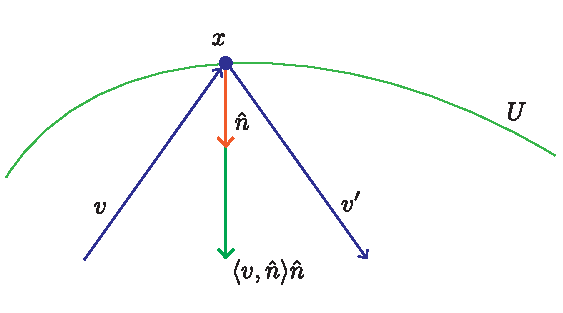
\includegraphics[width=.8\textwidth]{./figures/extra/bounce-bps}
	\caption{\label{fig:bounce-bps}Illustration of the specular reflection. The new velocity vector $v'$ is obtained by doing a specular reflection of the old vector $v$ against the level set of $U$ passing by $x$ (green line). This is obtained by subtracting twice the projection (green arrow) of the velocity on the normal vector to $U$ at $x$ (orange arrow). Figure best seen in colour.}
\end{figure}
%
%\clearpage

The authors show that the velocities also need to be ``refreshed'' according to the arrival times of a (homogenous) Poisson process (PP) of intensity $\lambda^{\text{ref}}\ge 0$, a parameter of the BPS. This ensures the algorithm explores the entirety of the space. The basic BPS algorithm is reproduced in \hyperref[alg:BPS1]{algorithm~\ref*{alg:BPS1}} below.

%\clearpage

\begin{algorithm}[!h]\small
	\caption{\label{alg:BPS1}\small \idblue{Basic BPS}}
	\begin{algorithmic}[1]
	\State initialise $(x^{(0)},v^{(0)})$, set $T$, trajectory length, set $t=0$ and $i=1$
	\While{$t < T$}
		\State simulate first arrival time $\tau_{\text{bounce}} \sim \text{PP}(\chi(t))$  with
		$$ \chi(t) = \lambda(x^{(i-1)}+v^{(i-1)}t,v^{(i-1)})$$
		\State simulate $\tau_{\text{ref}}\sim \mathrm{Exp}(\lambda^{\text{ref}})$
		\State let $\tau_{i}\leftarrow \min(\tau_{\text{bounce}},\tau_{\text{ref}})$
		\State compute the next position $x^{(i)}\leftarrow x^{(i-1)}+v^{(i-1)}\tau_{i}$
		\If{$\tau_{i}=\tau_{\text{ref}}$}
			\State sample next velocity $v^{(i)}\sim \mathcal N(0,I)$		\ElsIf{$\tau_{i}=\tau_{\text{bounce}}$}
			\State reflect the velocity $v^{(i)}\leftarrow R(x^{(i)})v^{(i-1)}$
		\EndIf
		\State let $t\leftarrow t_{i}\leftarrow t_{i-1}+\tau_{i}$
		\State update $i\leftarrow i+1$
	\EndWhile
	\end{algorithmic}
\end{algorithm}

The process for two subsequent time steps is illustrated at the figure \ref{fig:bps-trajec} below.
\begin{figure}[!h]
\center
	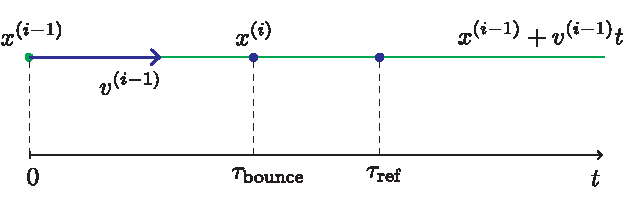
\includegraphics[width=.8\textwidth]{./figures/extra/trajec-bps}
	\caption{\label{fig:bps-trajec} Illustration of the process to go from $x^{(i-1)}$ to $x^{(i)}$ in the BPS: a bouncing time $\tau_{\text{bounce}}$ is drawn from the IPP with intensity $\chi(t)$ along the trajectory $x^{(i-1)}+v^{(i-1)}t$ (green line); a reference time $\tau_{\text{ref}}$ is drawn from an exponential, the minimum of the two (here $\tau_{\text{bounce}}$) leads to the position of the next point $x^{(i)}$ where either a bounce or a refreshment of the velocity will happen (here a bounce). Figure best seen in colour.}
\end{figure}
%\clearpage

As we saw, the algorithm requires to sample the first arrival time of an IPP of intensity $\chi(t)=\lambda(x+vt,v)$ where $\lambda(x,v)=\scal{\nabla U(x),v}^{+}$. Sampling from an IPP is a well explored topic in the literature and the authors summarise three possible approaches which we list briefly below:
\begin{itemize}\itsep0
	\item   \emph{Time-scale transformation}: this approach requires computing the inverse quantile of $\Xi(t):=\int_{0}^{t} \chi(s)\mathrm{d}s$ which is usually intractable but it can be computed numerically if the target is strictly log-concave and differentiable. Given $V$ drawn from a Uniform on $[0,1]$, the first arrival time of the IPP is given by $\Xi^{\inv}(-\log(V))$.
%This, the authors show, allows to make a connection with the Metropolis Hastings algorithm.
 \item   \emph{Adaptive thinning}: this approach requires an upper bounds $\overline{\chi}_{s}(t)$ with $\overline\chi_{s}(t)=0$ for $t<s$ and $\overline\chi_{s}(t)\ge\chi(t)$ for $s\le t\le s+\Delta(s)$ where $\Delta$ is a positive function (in the standard case, $\Delta=+\infty$). Additionally, it requires the ability to sample from the IPP corresponding to $\overline\chi_{s}$. Let $\tau$ be such a sample with $\tau\le s+\Delta$, there is then an accept-reject step with rate $\chi(\tau)/\overline\chi(\tau)$. Ideally, $\Delta$ and $\chi/\overline\chi_{s}$ are large (so that we do not have to simulate too many candidates which would incur an increased computational cost).
 \item   \emph{Superposition}: if the energy $U$ can be decomposed in a sum $U(x)=\sum_{j=1}^{m}U^{[j]}(x)$ and that each term can be targeted (via one of the first two methods), then we can use the thinning method with bound $\sum_{j=1}^{m}\chi^{[j]}(t)$.
 \end{itemize}
The key elements when trying to deploy the Bouncy Particle Sampler in practice are to select an appropriate $\lambda_{\text{ref}}$ (too low and the processus is essentially a random walk, too high and some regions of space may be left unexplored for a long time) and to implement an appropriate way to sample the first arrival time of the IPP which will depend on the target distribution.

An advantage of the BPS over methods such as HMC is that it can work seamlessly on constrained domains as is shown in \citet{bierkens17}.


%\section{Discussion}
%
%\todofr{
%\textbf{move this discussion where it belongs: at end of content chapters}
%	Connect the two background sections with main element (PF, PS link to HMM, PDMP, Local PDMP for anything. Exact methods.).
%}


